\chapter{Display}
\label{ch:display}
The display screen is the most important part of the interface presented by a personal workstation
to its users. At first sight, it simply represents a rectangular output area. However, in combination
with the mouse, it quickly develops into a sophisticated interactive input/output platform of almost
unlimited flexibility. It is mainly its Janus-faced characteristic that makes the display screen stand
out from ordinary external devices to be managed by the OS. In the current chapter
we shall give more detailed insight into the reasons for central position that the display system
takes within the OS, and for its determining influence on the entire system architecture. In particular,
we shall show that the display system is a natural basis or anchor for functional extensibility.

\section{Screen Layout Model}
In the early seventies, Xerox PARC in California launched the Smalltalk project with the goal of
conceiving and developing new more natural ways to communicate with personal computers\cite{Goldberg}.
Perhaps the most conspicuous among several significant achievements of this endeavor is the idea of 
applying the desktop metaphor to the display screen. This metaphor comprises a desktop and the collection
of possibly mutually overlapping pages of paper that are laid out on the desktop. By projecting such a
configuration onto the surface of a screen we get the familiar picture of Fig \ref{fig:desktop} showing
a collection of partially or totally visible rectangular areas on a background, so-called windows or viewers.
\begin{figure}
	\centering
	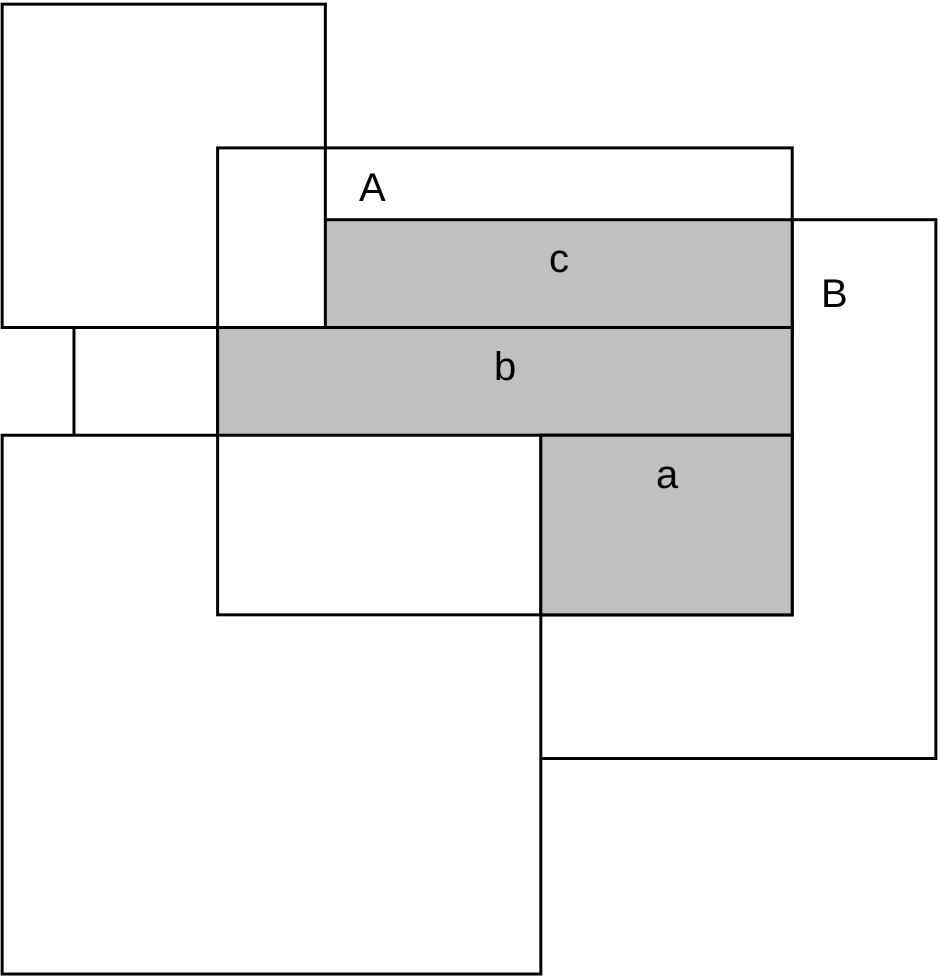
\includegraphics[width=.6\textwidth]{i/4}
	\caption{Desktop showing partially overlapping viewers}
	\label{fig:desktop}
\end{figure}

The desktop metaphor is used by many modern OSes and user interface shells both
as a natural model for the system to separate displayed data belonging to different tasks, and as a
powerful tool for users to organize the display screen interactively, according to individual taste
and preference. However, there are inherent drawbacks in the metaphor. They are primarily
connected with overlapping. Firstly, any efficient management of overlapping viewers must rely on
a subordinate management of (arbitrary) sub-rectangles and on sophisticated clipping operations.
This is so because partially overlapped viewers must be partially restored under control of the
viewer manager. For example, in Fig \ref{fig:desktop}, rectangles $a$, $b$, and $c$ in viewer $B$ ought 
to be restored individually after closing of $A$. Secondly, there is a significant danger of covering
viewers completely and losing them forever. And thirdly, no canonical heuristic algorithms exist for
automatic allocation of screen space to newly opened viewers.

Experience has shown that partial overlapping is desirable and beneficial in rare cases only, and
so the additional complexity of its management \cite{Binding, Wille} is hard to justify. Therefore,
alternate strategies to structure a display screen have been looked for. An interesting class of
established solutions can be titled as \textbf{tiling}. There are several variants of it \cite{Cohen}. 
Perhaps the most obvious one (because the most unconstrained one) is based on iterated horizontal or
vertical splitting of existing viewers. Starting with the full screen and successively opening
$A$, $B$, $C$, $D$, $E$, and $F$ we get to a configuration as in Fig \ref{fig:tiling}.
\begin{figure}
	\centering
	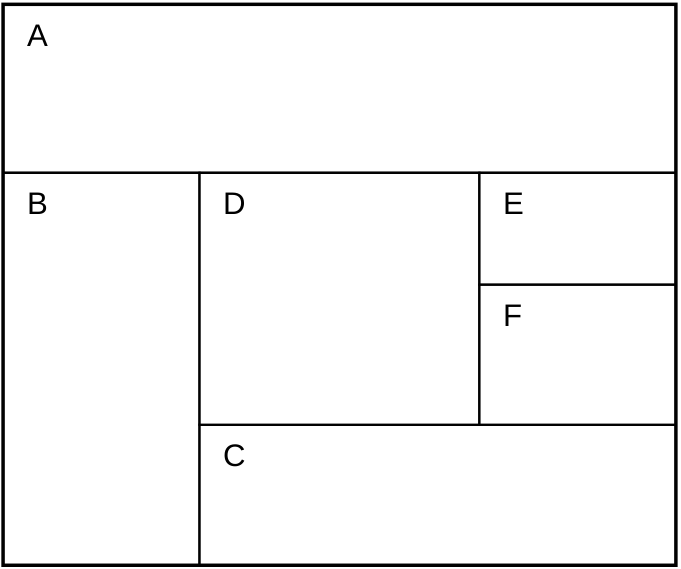
\includegraphics[width=.6\textwidth]{i/5}
	\caption{Viewer configuration resulting from unconstrained tiling}
	\label{fig:tiling}
\end{figure}
A second variant is hierarchic tiling. Again, the hierarchy starts with a full screen that is now
decomposed into a number of vertical tracks, each of which is further decomposed into a number
of horizontal viewers. We decided in favor of this kind of tiling in Oberon, mainly because the
algorithm of reusing the area of a closed viewer is simpler and more uniform. For example,
assume that in Fig \ref{fig:tiling} viewer $F$ has been closed. Then, it is straightforward to reverse the
previous opening operation by extending viewer $E$ at its bottom end. However, if the closed viewer
is $B$, no such simple procedure exists. For example, the freed area can be shared between
viewers $C$ and $D$ by making them extend to their left. Clearly, no such complicated situations can
occur in the case of hierarchic tiling.

Hierarchic tiling is also used in Xerox PARC's Cedar system \cite{Teitelman}. However, the Oberon
variant differs from the Cedar variant in some respects. Firstly, Oberon supports quick temporary
context switching by overlaying one track or any contiguous sequence of tracks with new layers.
In Fig \ref{fig:overlay} a snapshot of a standard Oberon display screen is graphically represented. It
\begin{figure}
	\centering
	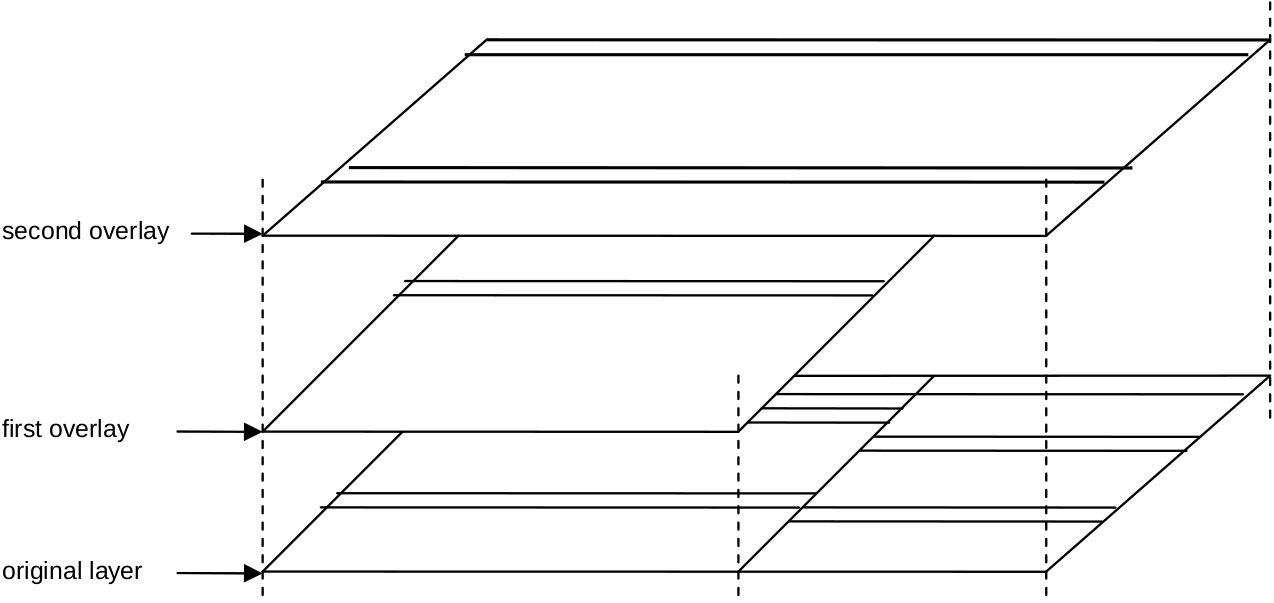
\includegraphics[width=\textwidth]{i/6}
	\caption{Overlay of tracks and sequences of tracks}
	\label{fig:overlay}
\end{figure}
suggests two original tracks and two levels of overlay, where the top layer is screen-filling.
Secondly, unlike Cedar display screens, Oberon displays do not provide reserved areas for
system-wide facilities, Standard Cedar screens feature a command row at the top and an icon row
at the bottom. And thirdly, Oberon is based on a different heuristic strategy for the automatic
placement of new viewers. As a Cedar default invariant, the area of every track is divided up
evenly among the viewers in this track. When a new viewer is to be placed, the existing viewers in
the track are requested to reduce their size and move up appropriately. The newly opened viewer
is then allocated in the freed spot at the bottom. In contrast, Oberon normally splits the largest
existing viewer in a given track into two halves of equal size. As an advantage of this latter
allocation strategy we note that existing contents are kept stable.

\section{Viewers as Objects}
Although everybody seems to agree on the meaning of the term viewer, no two different system
designers actually do. The original role of a viewer as merely a separate display area has
meanwhile become heavily overloaded with additional functionality. Depending on the underlying
system are viewers' individual views on a certain configuration of objects, carriers of tasks,
processes, applications, etc. Therefore, we first need to define our own precise understanding of
the concept of viewer.

The best guide to this aim is the abstract data type $Viewer$ that we introduced in Chapter 3. We
recapitulate: type $Viewer$ serves as a template describing viewers abstractly as “black boxes” in
terms of a state of visibility, a rectangle on the display screen, and a message handler. The exact
functional interface provided by a given variant of viewer is determined by the set of messages
accepted. This set is structured as a customized hierarchy of type extensions.

We can now obtain a more concrete specification of the role of viewer by identifying some basic
categories of universal messages that are expected to be accepted by all variants of viewer. For
example, we know that messages reporting about user interactions as well as messages defining
a generic operation are universal. These two categories of universal messages document the
roles of viewers as interactive tasks and as parts of an integrated system respectively.
In total, there are four such categories. They are here listed together with the corresponding topic and message dispatchers:
\begin{table}[h!]
	\setlength{\tabcolsep}{1pt}
	\begin{tabular}{r|c|l}
		Dispatcher               &Topic
		                         &Message \\\hline
		{\small task scheduler } &{\small dispatching tasks       }
		                         &{\small report user interaction }\\
		{\small cmd interpreter} &{\small processing command      }
		                         &{\small define generic operation}\\
		{\small view manager   } &{\small organizing display area }
		                         &{\small location/size change    }\\
		{\small doc manager    } &{\small operating on document   }
		                         &{\small content/format change   }
	\end{tabular}
\end{table}
These topics essentially define the role of viewers. In short, we may look at an Oberon viewer as a non-overlapped rectangular box on the screen both acting as an integrated display area for some objects of a document and representing an interactive task in the form of a sensitive
editing area.

Shifting emphasis a little and regarding the various message dispatchers as subsystems, we
recognize immediately the role of viewers as integrator of the different subsystems via message-based interfaces. In this light type $Viewer$ appears as a common object-oriented basis of Oberon's
subsystems.

The topics listed above constitute some kind of contents backbone of the \ref{ch:task}, \ref{ch:display} 
and \ref{ch:text}. Task scheduling and command interpreting are already familiar to us from \textsection 3.2 and 3.3. Viewer and text management will be the topics of \textsection 4.4 and 5.2, respectively.
Thereby, the built-in type $Text$ will serve as a prime example of a document type.
The activities that a viewer performs are basically controlled by events or, more precisely, by
messages representing event notices. We shall explain this in \textsection 4.4 and 5.3 in detail cases of an abstract class of standard viewers and a class of viewers displaying standard text, respectively.

Here is a preliminary overview of some archetypal kinds of message:
\begin{itemize}
	\item After each key stroke a keyboard message containing the typed character is sent to the current focus viewer and after each mouse click a mouse message reporting the new state of the mouse is sent to the viewer containing the current mouse position.
	\item A message often represents some generic operation that is expected to be interpreted individually by its recipients. Obvious examples in our context are "return current textual selection", "copy-over stretch of text", and "produce a copy (clone)". Notice that generic operations are the key to extensibility.
	\item In a tiling viewer environment, every opening of a new viewer and every change of size or location of an existing viewer has an obvious effect on adjacent viewers. The viewer manager therefore issues a message for every affected viewer requesting it to adjust its size appropriately.
	\item Whenever the contents or the format of a document has changed, a message notifying all visible viewers of the change is broadcast. Notice that broadcasting messages by a model (document) to the entirety of its potential views (viewers) is an interesting implementation of the famous MVC (model-view-controller) pattern that dispenses models from “knowing” (registering) their views.
\end{itemize}

\section{Frames as Basic Display Entities}
When we introduced viewers in Chapter 3 and the previous section, we simplified with the aim of abstraction. We know already that viewers appear as elements of second order in the tiling hierarchy. Having treated them as black boxes so far we have not revealed anything about the hierarchy continuation. As a matter of fact, viewers are neither elementary display entities nor atoms. They are just a special case of so-called [display] frames. They are arbitrary rectangles displaying a collection of objects or a document excerpt. In particular, they may recursively contain other frames, a capability that makes them an
extremely powerful tool for any display organizer.

The type $Frame$ is declared as
\begin{verbatim}
  Frame = POINTER TO FrameDesc;
  FrameDesc = RECORD
    next, dsc: Frame;
    X, Y, W, H: INT;
    handle: Handler
  END;
\end{verbatim}

The components $next$ and $dsc$ are connections to further frames. Their names suggest a multilevel recursive hierarchical structure: $next$ points to the next frame on the same level, while $dsc$
points to the (first) descendant, i.e. to the next lower level of the nested frames hierarchy. $X$, $Y$, $W$, $H$, and the handler $handle$ serve the original purpose to that we introduced them. In particular,
the handler allows frames to react individually on the receipt of messages. Its type is
\begin{verbatim}
  Handler = PROC (F: Frame; VAR M: FrameMsg);
\end{verbatim}
where $FrameMsg$ represents the root of a potentially unlimited tree hierarchy of possible messages to frames:
\begin{verbatim}
  FrameMsg = RECORD END;
\end{verbatim}
Having now introduced the concept of frames, we can reveal the whole truth about viewers. As a matter of fact, type $Viewer$ is a derived type, it is a type extension of $Frame$:
\begin{verbatim}
  Viewer = POINTER TO ViewerDesc;
  ViewerDesc = RECORD (FrameDesc)
    state: INT
  END;
\end{verbatim}
These declarations formally express the fact that viewers are nothing but a special case (or
variant or subclass) of general frames, additionally featuring a state of visibility. In particular,
viewers inherit the hierarchical structure of frames. This is an extremely useful property
immediately opening an unlimited spectrum of possibilities for designers of a specific subclass of
viewers to organize the representing rectangular area. For example, the area of viewers of, say,
class $Desktop$ may take the role of a background being covered by an arbitrary collection of
possibly mutually overlapping frames. In other words, our decision of using a tiling viewer scheme
globally can easily be overwritten locally.

An even more important example of a predefined structure is provided by the abstract class of socalled menu viewers whose shape is familiar from most snapshots taken of the standard Oberon
display screen. A menu viewer consists of a thin rectangular boundary line and an interior area
being vertically decomposed into a menu region at the top and a contents region at the bottom (see Fig \ref{fig:menu}).
\begin{figure}
	\centering
	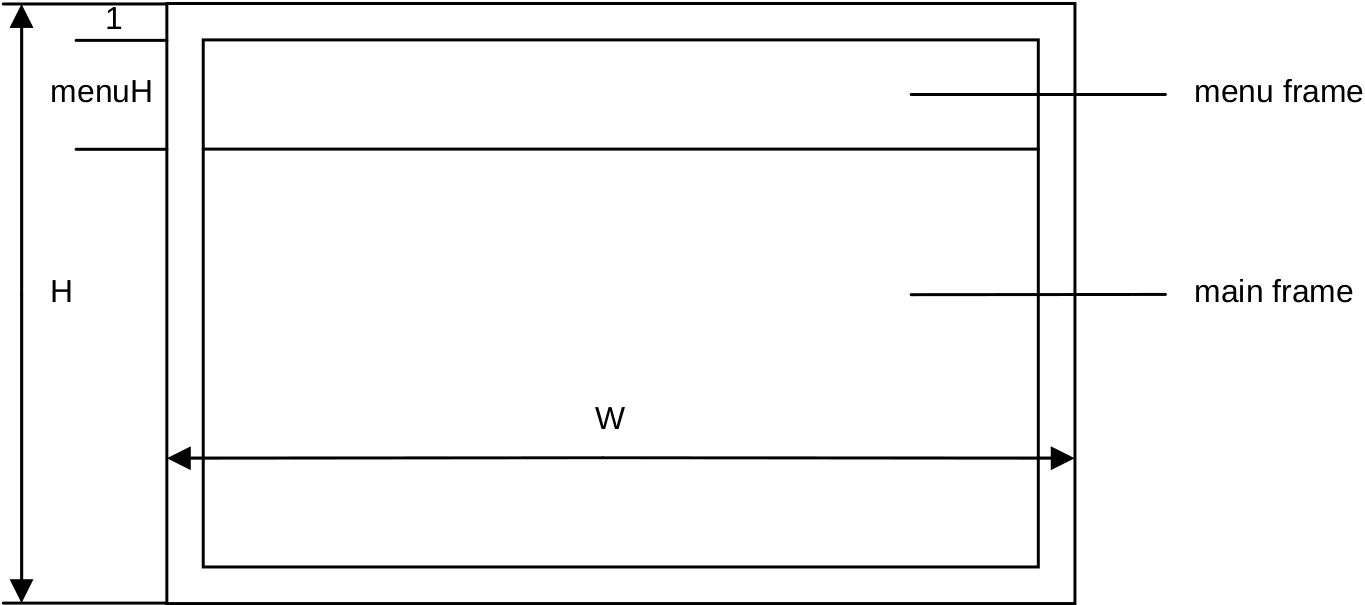
\includegraphics[width=\textwidth]{i/7}
	\caption{The compositional structure of a menu viewer}
	\label{fig:menu}
\end{figure}

In terms of data structures, the class of menu viewers is defined as a type extension of $Viewer$ with an additional component $menuH$ specifying the menu frame height:
\begin{verbatim}
  MenuViewer = POINTER TO MenuViewerDesc;
  MenuViewerDesc = RECORD (ViewerDesc)
    menuH: INT
  END;
\end{verbatim}
Each menu viewer $V$ specifies exactly two descendants: the menu frame $V.dsc$ and the frame of main contents or main frame $V.dsc.next$. Absolutely nothing is fixed about the two descendant frames contents. In the standard case, however, the menu frame is a text frame, displaying a line of commands in inverse video mode. By definition, the main frame nature specifies the viewer type. If it is a text frame as well, then we call the viewer a text one, if a graphics frame, we call it a graphics viewer etc.

\section{Display management}
Oberon's display system comprises two main topics: viewer management and cursor handling.
Let us first turn to the much more involved topic of viewer management and postpone cursor
handling to the end of this section. Before we can actually begin our explanations we need to
introduce the concept of the logical display area. It is modeled as a two-dimensional Cartesian
plane housing the totality of objects to be displayed. The essential point of this abstraction is a
rigorous decoupling of any aspects of physical display devices. As a matter of fact, any concrete
assignment of display monitors to certain finite regions of the display area is a pure matter of
configuring the system.

Being a subsystem of OS with well-defined modular structure, the display system appears
in the form of a small hierarchy of modules. Its core is a linearly ordered set consisting of three
modules: $Display$, $Viewer$s, and $MenuViewer$s, the latter building upon the former. Conceptually,
each module contributes an associated class of display-oriented objects and a collection of related service routines.

The following is an overview of the subsystem viewer management. Modules on upper lines import lower ones and types on upper lines extend those on lower.
\begin{table}[h!]
	\setlength{\tabcolsep}{2pt}
	\begin{tabular}{l|l|l}
		Module     &Type   &Service \\\hline
		MenuViewer &Viewer &Message handling for menu viewers\\
		Viewers    &Viewer &Tiling viewer management\\
		Display    &Frame  &Block-oriented raster operations
	\end{tabular}
\end{table}
Inspecting the column titled $Type$ we recognize precisely our familiar types $Frame$, $Viewer$, and
$MenuViewer$ respectively, where the latter is an abbreviation of $MenuViewers.Viewer$.
In addition to the core modules of the display system a section in module $Oberon$ provides a
specialized application programming interface (API) that simplifies the use of the viewer
management package by applications in the case of standard Oberon display configurations. We
shall come back to this topic in Section 4.6.

For the moment let us concentrate on the core of viewer management and in particular on the
modules $Viewer$s and $MenuViewer$s, saving the discussion of module $Display$ for the next
section. Typically, we start the presentation of a module by listing and commenting its definition,
and we refer to subsequent listings for its implementation.

\subsection{Viewers}
Focusing first on module $Viewer$s we can roughly define the domain of its responsibility as
"initializing and maintaining the global layout of the display area". From the previous discussion
we are well acquainted already with the structure of the global display space as well as its
building blocks: the display area is hierarchically tiled with display frames, where the first two
levels in the frame hierarchy correspond to tracks and viewers respectively.

This is the formal definition:
\begin{verbatim}
  DEFINITION Viewers;
    IMPORT Display;

    (*message ids*)
    CONST restore = 0; modify  = 1; suspend = 2;
    TYPE Viewer = POINTER TO ViewerDesc;
    ViewerDesc = RECORD (Display.FrameDesc)
      state: INT
    END;
  
    ViewerMsg = RECORD (Display.FrameMsg)
      id: INT;
      X, Y, W, H: INT;
      state: INT
    END;
    VAR curW: INT;

    (*track handling*)
    PROC InitTrack (W, H: INT;
                         Filler: Viewer);
    PROC OpenTrack (X, W: INT;
                         Filler: Viewer);
    PROC CloseTrack (X: INT);

    (*viewer handling*)
    PROC Open (V: Viewer; X, Y: INT);
    PROC Change (V: Viewer; Y: INT);
    PROC Close (V: Viewer);

    (*miscellaneous*)
    PROC This (X, Y: INT): Viewer;
    PROC Next (V: Viewer): Viewer;
    PROC Recall (VAR V: Viewer);
    PROC Locate (X, H: INT;
                   VAR fil, bot, alt, max: Viewer);
    PROC Broadcast (VAR M: Display.FrameMsg);
  END Viewers.
\end{verbatim}

Some comments: a first group of procedures consisting of $InitTrack$, $OpenTrack$, and $CloseTrack$
supports the track structure of the display area. $InitTrack$ creates a new track of width $W$ and
height $H$ by partitioning off a vertical strip of width $W$ from the display area. In addition, $InitTrack$
initializes the newly created track with a filler viewer that is supplied as a parameter. The filler
viewer essentially serves as background filling up the track at its top end. It reduces to height 0 if
the track is covered completely by productive viewers.

Configuring the display area is part of system initialization after startup. It amounts to executing a sequence of steps in the form
\begin{verbatim}
  NEW(Filler);
  Filler.handle := HandleFiller;
  InitTrack(W, H, Filler)
\end{verbatim}
where $HandleFiller$ is supposed to handle messages that require modifications of size and cursor
drawing.

The global variable $curW$ indicates the already configured part width of the display area.
Note that configuring starts with $x = 0$ and is non-reversible in sense that the grid defined by
the initialized tracks cannot be refined later. However, remember that it can be coarsened at any
time by overlaying a contiguous sequence of existing tracks by a single new track.

Procedure $OpenTrack$ serves exactly this purpose. The track (or sequence of tracks) to be
overlaid in the display-area must be spanned by the segment $[X, X + W)$. Procedure $CloseTrack$ is
inverse to $OpenTrack$. It is called to close the (topmost) track located at $X$ in the display area, and
to restore the previously covered track (or sequence of tracks).

The next three procedures are used to organize viewers within individual tracks. Procedure $Open$
allocates a given viewer at a given position. More precisely, $Open$ locates the viewer containing
point $(X, Y)$, splits it horizontally at height $Y$, and opens the viewer $V$ in the lower part of area. In the special case of $Y$ coinciding with the upper boundary line of the located viewer this is
closed automatically. Procedure $Change$ allows to change the height of a given viewer $V$ by
moving its upper boundary line to a new location $Y$ (within the limits of its neighbors). Procedure
$Close$ removes the given viewer $V$ from the display area. Fig \ref{fig:operation} makes these operations clear.
\begin{figure}
	\centering
	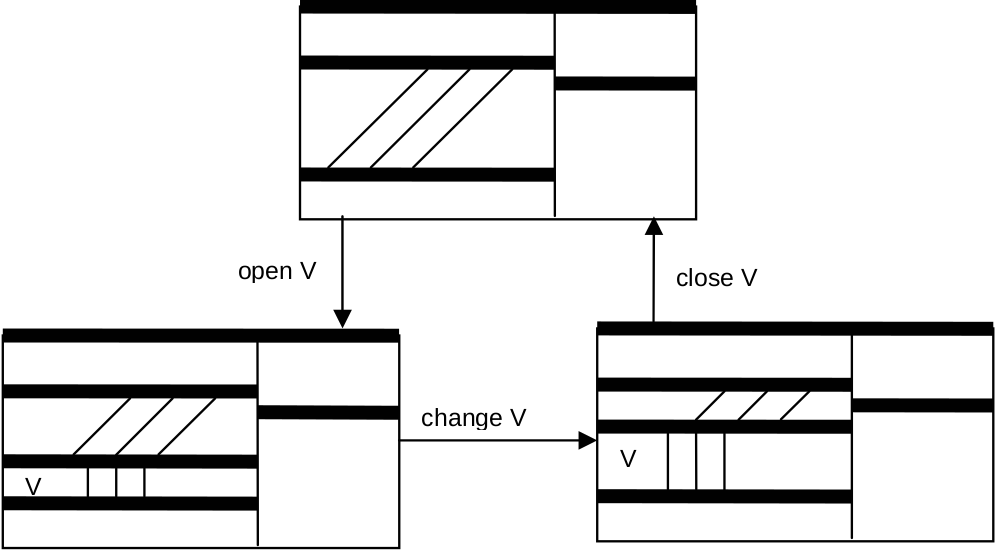
\includegraphics[width=\textwidth]{i/8}
	\caption{Basic operations on viewers}
	\label{fig:operation}
\end{figure}

The last group of procedures provides miscellaneous services. Procedure $This$ identifies the
viewer displayed at $(X, Y)$. Procedure $Next$ returns the next upper neighbor of a given displayed
viewer $V$. Procedure $Recall$ allows recalling and restoring the most recently closed viewer. $Locate$
is a procedure that assists heuristic allocation of new viewers. For any given track and desired
minimum height, procedure $Locate$ offers a choice of some distinguished viewers in this track: the
filler viewer, the one at bottom, an alternative choice, and the viewer of maximum height.
Finally, procedure $Broadcast$ broadcasts a message to the display area, that is, sends the given
message to all viewers that are currently displayed.

It is now a good time to throw a glance behind the scenes. Let us start with revealing module
$Viewer$’s internal data structure. Remember that according to the principle of information hiding an
internal data structure is fully private to the containing module and accessible through the
module’s procedural interface only. Fig \ref{fig:snapshot} shows a data structure view of the display snapshot
taken in Fig \ref{fig:overlay}. Note that the overlaid tracks and viewers are still part of the internal data structure.

In the data structure we recognize an anchor that represents the display area and points to a list
of tracks, each of them in turn pointing to a list of viewers, each of them in turn pointing to a list of
arbitrary sub-frames. Both the list of tracks and the list of viewers are closed to a ring, where the
filler track (filling up the display area) and the filler viewers (filling up the tracks) act as anchors.
Additionally, each track points to a (possibly empty) list of tracks lying underneath. These frames
are invisible on the display, and shaded in Fig \ref{fig:snapshot}.
\begin{figure}
	\centering
	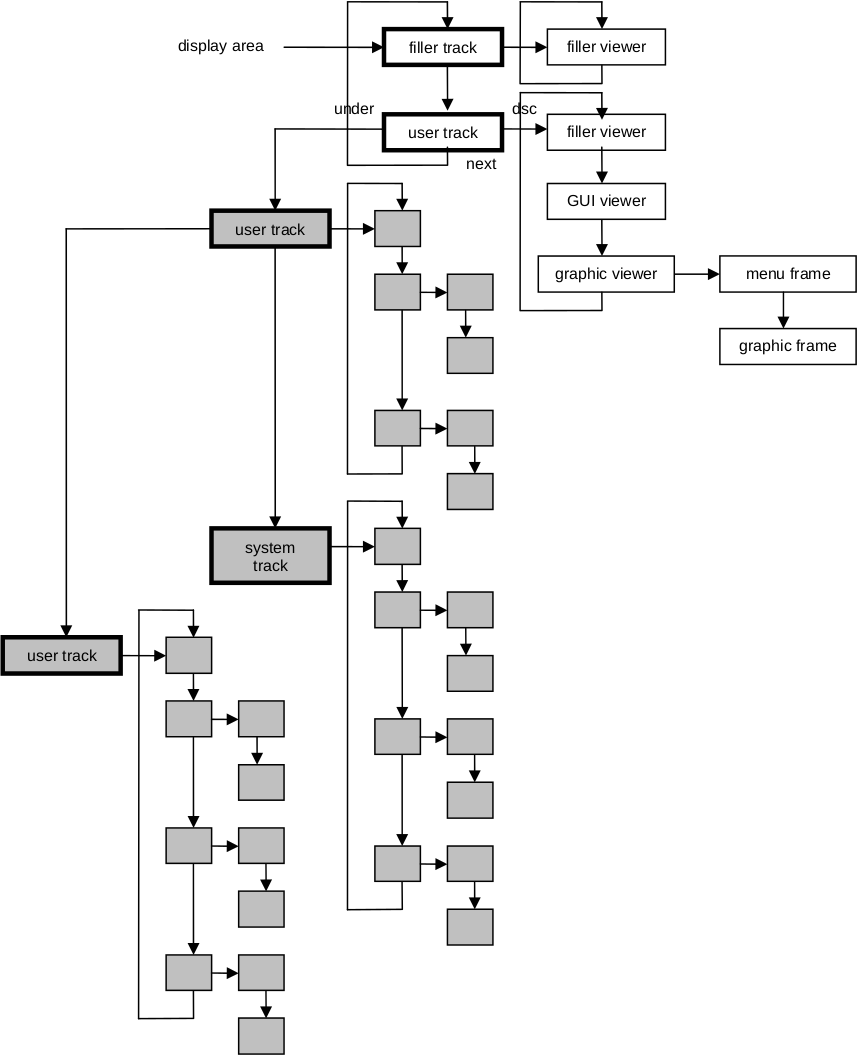
\includegraphics[width=\textwidth]{i/9}
	\caption{Internal data structure snapshot of Fig \ref{fig:overlay}}
	\label{fig:snapshot}
\end{figure}

Technically, the track descriptor type $TrackDesc$ is a private extension of the viewer descriptor
type $ViewerDesc$. Repeating the declarations of viewer descriptors and frame descriptors, we get to this hierarchy of types:
\begin{verbatim}
  TrackDesc = RECORD (ViewerDesc)
    under: Display.Frame
  END;

  ViewerDesc = RECORD (FrameDesc)
    state: INT
  END;

  FrameDesc = RECORD
    next, dsc: Frame;
    X, Y, W, H: INT;
    handle: Handler
  END;
\end{verbatim}

It is noteworthy that the data structure of the viewer manager is heterogeneous with $Frame$ as
base type. It provides a nice example of a nested hierarchy of frames with the additional property
that the first two levels correspond to the first two levels in the type hierarchy defined by $Track$,
$Viewer$, and $Frame$.

In an object-oriented environment objects are autonomous entities in principle. However, they may
be bound to some higher instance (other than the system) temporarily. For example, we can look
at the objects belonging to a module's private data structure as bound to this module. Deciding if
an object is currently bound then becomes a fundamental problem. In the case of viewers, this
information is contained in an extra instance variable called state.

As a system invariant, we have for every viewer $V$
\[ V\text{ is bound to module }Viewers \Leftrightarrow V.state \neq 0 \]
If we call any displayed viewer $visible$ and each that is covered by an overlaying track $suspended$, we can refine this invariant to
\begin{align*}
&\{ V\text{ is }visible  \Leftrightarrow V.state > 0 \}\text{ and }\\
&\{ V\text{ is }suspended\Leftrightarrow V.state < 0 \}
\end{align*}
In addition, more detailed information about the kind of viewer $V$ is given by the magnitude $|V.state|$:
\begin{table}[h!]
	\centering
	\begin{tabular}{r l}
		$V.state$ & kind of viewer \\\hline
		        0 & closed \\
		        1 & filler \\
		       -1 & productive
	\end{tabular}
\end{table}
The magnitude $|V.state|$ is kept invariant by module $Viewers$. It could be used, for example, to
distinguish different levels of importance or preference with the aim of supporting a smarter
algorithm for heuristic allocation of new viewers. The variable state is treated as read-only by
every module other than $Viewers$.

We are now sufficiently prepared to understand how the exported procedures of module $Viewers$
work behind the scenes. All of them operate on the internal dynamic data structure just explained.
Some use it as a reference only or operate on individual elements (procedures $This$,
$Next$, $Locate$, $Change$), others add new elements to it (procedures $InitTrack$,
$OpenTrack$, $Open$), and even others remove elements (procedures $CloseTrack$, $Close$). Most
of them have side-effects on the size or state of existing elements.

Let us now change perspective and look at module $Viewers$ as a general low-level manager of
viewers whose exact contents are unknown to it (and whose controlling software might have been
developed years later). In short, let us look at module $Viewers$ as a manager of black boxes. Such
an abstraction immediately makes it impossible for the implementation to call fixed procedures for,
say, changing a viewer's size or state. The facility needed is a message-oriented interface.
\begin{verbatim}
  TYPE ViewerMsg = RECORD (Display.FrameMsg)
    id: INT;
    X, Y, W, H: INT;
    state: INT
  END;
\end{verbatim}

There exist three variants of $Viewer$ messages, discriminated by the field $id$: restore contents,
modify height (extend or reduce at bottom), and suspend (close temporarily or permanently). The
additional components of the message inform about the desired new location, size, and state.
The following table lists senders, messages, and recipients of viewer messages.
\begin{table}[h!]
	\setlength{\tabcolsep}{1pt}
	\begin{tabular}{l|l|l}
		Originator         &Message                 &Recipients \\\hline
		{\small OpenTrack }&{\small suspend temporarily}
		                   &{\small viewers covered by opening track }\\
		{\small CloseTrack}&{\small suspend permanently}
		                   &{\small viewers in closing track         }\\
		{\small Open      }&{\small modify or suspend  }
		                   &{\small upper neighbor of opening viewer }\\
		{\small Change    }&{\small modify             }
		                   &{\small upper neighbor of changing viewer}\\
		{\small Close     }&{\small suspend permanently}
		                   &{\small closing viewer                   }
	\end{tabular}
\end{table}

\subsection{Menu Viewers}
So far, we have treated viewers abstractly as black boxes. Our next step is now to focus on a
special class of viewers called menu viewers. Remembering the definition given earlier we know
that a menu viewer is characterized by a structure consisting of two vertically tiled “descendant”
frames, a menu frame at the top and a frame of contents at the bottom. Because the nature and
contents of these frames are typically unknown by their “ancestor” (or “parent”) viewer, a collection
of abstract messages is again a postulating form of interface. As net effect, the handling of menu
viewers boils down to a combination of preprocessing, transforming and forwarding messages to
the descendant frames. In short, the display space in Oberon is hierarchically organized and
message passing within the display space obeys the pattern of strict parental control.

Again, we start our more detailed discussion with a module interface definition:
\begin{verbatim}
  DEFINITION MenuViewers;
    IMPORT Viewers, Display;
    CONST extend = 0; reduce = 1; move = 2;
                                  (*message ids*)
    TYPE Viewer = POINTER TO ViewerDesc;
    ViewerDesc = RECORD (Viewers.ViewerDesc)
      menuH: INT
    END;

    ModifyMsg = RECORD (Display.FrameMsg)
      id: INT;
      dY, Y, H: INT
    END;

    PROC Handle (V: Display.Frame;
                      VAR M: Display.FrameMsg);
    PROC New (Menu, Main: Display.Frame;
                   menuH, X, Y: INT): Viewer;
  END MenuViewers.
\end{verbatim}
The interface represented by this definition is conspicuously narrow. There are just two
procedures: a generator procedure $New$ and a standard message handler $Handle$. The generator
returns a newly created menu viewer displaying the two (arbitrary) frames passed as parameters.
The message handler implements the entire “behavior” of an object and in particular the above
mentioned message dispatching functionality.

Message handlers in Oberon are implemented in the form of procedure variables that obviously
must be initialized properly at object creation time. In other words, some concrete behavior must
explicitly be bound to each object, where different instances of the same object type could
potentially have a different behavior and/or the same instance could change its behavior during its
lifetime. Our object model is therefore instance-centered.

Conceptually, the creation of an object is an atomic action consisting of three basic steps:
allocate memory block; install message handler; initialize state variables

In the case of a standard menu viewer $V$ this can be expressed as
\begin{verbatim}
  NEW(V); V.handle := Handle; V.dsc := Menu;
          V.dsc.next := Main; V.menuH := menuH
\end{verbatim}
With that, calling $New$ is equivalent with
\begin{verbatim}
  create V; open V at X, Y
\end{verbatim}
where opening $V$ needs assistance by module $Viewers$.

The implementation of procedure Handle embodies the standard strategy of message handling by
menu viewers. The following code is a coarse-grained view of it.
\begin{verbatim}
Message handler for menu viewers
IF message reports about user interaction THEN
  IF variant is mouse tracking THEN
    IF mouse is in menu region THEN
      IF mouse is in upper menu region and
                       left key is pressed THEN
        handle changing of viewer
      ELSE delegate handling to menu-frame
      END
    ELSE
      IF mouse is in main-frame THEN
        delegate handling to main-frame
      END
    END
  ELSIF variant is keyboard input THEN
    delegate handling to menu frame;
    delegate handling to main frame
  END
ELSIF message defines generic operation THEN
  IF message requests copy (clone) THEN
    send copy message to menu frame to get a copy;
    send copy message to main frame to get a copy;
    create menu viewer clone from copies
  ELSE
    delegate handling to menu frame;
    delegate handling to main frame
  END
ELSIF message reports about change of contents THEN
  delegate handling to menu frame;
  delegate handling to main frame
ELSIF message requests change of location/size THEN
  IF operation is restore THEN
    draw viewer area and border;
    send menu frm modify msg to make extend from H 0;
    send main frm modify msg to make extend from H 0
  ELSIF operation is modify THEN
    IF operation is extend THEN
      extend viewer area and border;
      send modify msg to menu frm to make it extend;
      send modify msg to main frm to make it extend
    ELSE (*reduce*)
      send modify msg to main frm to make it reduce;
      send modify msg to menu frm to make it reduce;
      reduce viewer area and border
    END
  ELSIF operation is suspend THEN
    send main frm modify msg to make reduce to H 0;
    send menu frm modify msg to make reduce to H 0
  END
END
\end{verbatim}

In principle, the handler acts as a message dispatcher that either processes a message directly
and/or delegates its processing to the descendant frames. Note that the handler's main alternative
statement discriminates precisely among the four basic categories of messages.

From the above outlined algorithm handling copy messages, that is, requests for generating a
copy or clone of a menu viewer, we can derive a general recursive scheme for the creation of a
clone of an arbitrary frame:

send copy message to each element in the list of descendants;
generate copy of the original frame descriptor;
attach copies of descendants to the copy of descriptor

The essential point here is the use of new outgoing messages in order to process a given
incoming message. We can regard message processing as a transformation that maps incoming
messages into a set of outgoing messages, with possible side-effects. The simplest case of such
a transformation is known as delegation. In this case, the input message is simply passed on to
the descendant(s).

As a fine point we clarify that the above algorithm is designed to create a deep copy of a
composite object (a menu viewer in our case). If a shallow copy would be desired, the
descendants would not have to be copied, and the original descendants instead of their copies
would be attached to the copy of the composite object.

Another example of message handling is provided by mouse tracking. Assume that a mouse
message is received by a menu viewer while the mouse is located in the upper part of its menu
frame and the left mouse key is kept down. This means "change viewer's height by moving its top
line vertically". No message to express the required transformation of the sub-frames yet exists.
Consequently, module $MenuViewer$s takes advantage of our open (extensible) message model
and simply introduces an appropriate message type called $ModifyMsg$:
\begin{verbatim}
  ModifyMsg = RECORD (Display.FrameMsg)
    id: INT;
    dY, Y, H: INT
  END;
\end{verbatim}
The field $id$ specifies one of two variants: extend or reduce. The first variant of the message
requests the receiving frame to move by the vertical translation vector $dY$ and then to extend to
height $H$ at bottom. The second variant requests the frame to reduce to height $H$ at bottom and
then to move by $dY$. In both cases $Y$ indicates the Y-coordinate of the new lower-left corner.
Fig \ref{fig:modify} summarizes this graphically.
\begin{figure}
	\centering
	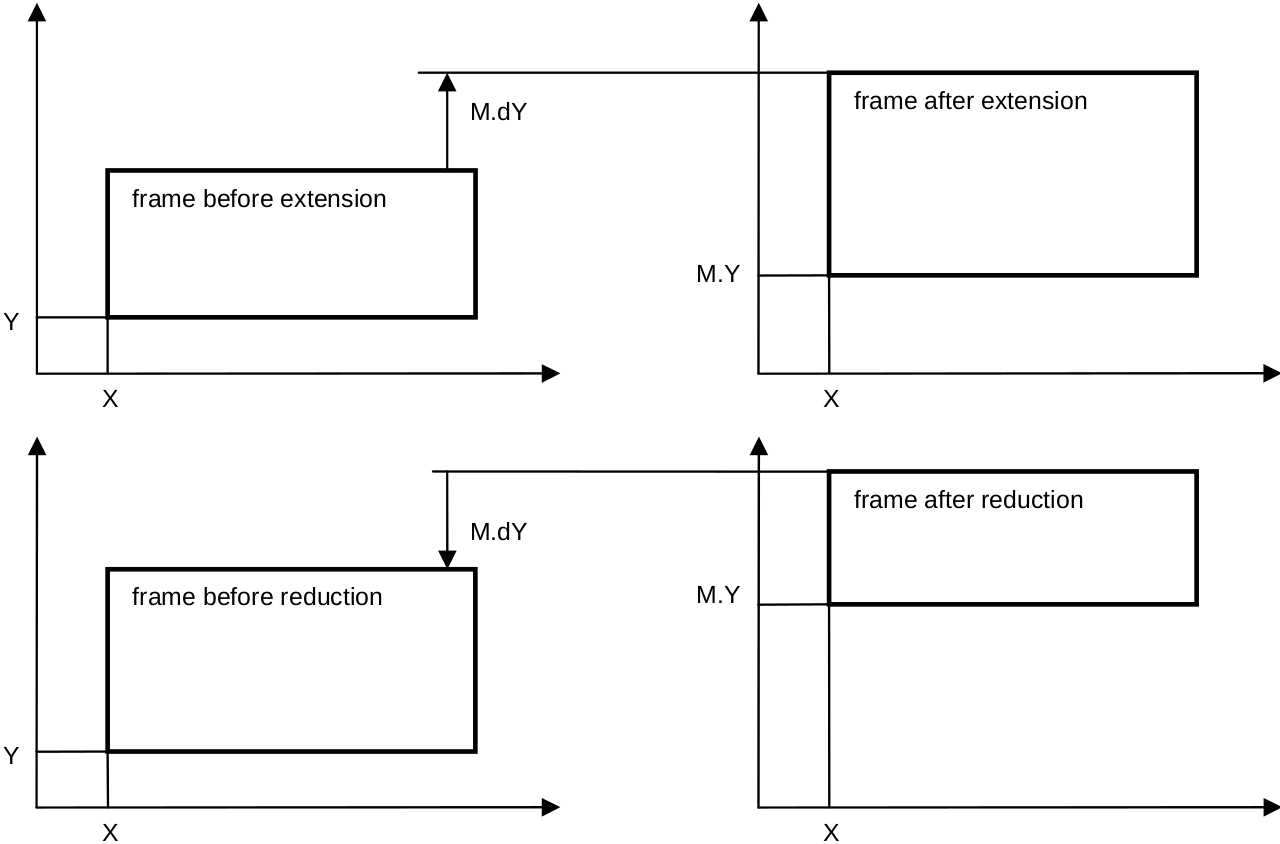
\includegraphics[width=\textwidth]{i/a}
	\caption{The modify frame operation}
	\label{fig:modify}
\end{figure}

Messages arriving from the viewer manager and requesting the receiving viewer to extend or
reduce at its bottom are also mapped into messages of type $ModifyMsg$. Of course, no translation
is needed in these cases, and dY is 0.

The attentive reader might perhaps have asked why the standard handler is exported by module
$MenuViewers$ at all. The thought behind is reusability of code. For example, a message handler
for a subclass of menu viewers could be implemented effectively by reusing menu viewer's
standard handler. After having handled all new or differing cases first it would simply (super-)call
the standard handler subsequently.

\subsection{Cursor Management}
Traditionally, a cursor indicates and visualizes on the screen the current location of the caret in a
text or, more generally, the current focus of attention. A small arrow or similar graphic symbol is
typically used for this purpose. In Oberon, we have slightly generalized and abstracted this
concept. A cursor is a path in the logical display area whose current position can be made visible
by a marker.

The viewer manager and the cursor handler are two concurrent users of the same display area.
Actually, we should imagine two parallel planes, one displaying viewers and the other displaying
cursors. If there is just one physical plane we take care of painting markers non-destructively, for
example in inverse-video mode. Then, no precondition must be established before drawing a
marker. However, in the case of a viewer task painting destructively in its viewer's area, the area
must be locked first after turning invisible all markers in the area.

The technical support of cursor management is again contained in module Oberon. The
corresponding application programming interface is
\begin{verbatim}
  DEFINITION Oberon;
    TYPE Marker = RECORD
      Fade, Draw: PROC (x, y: INT)
    END;

    Cursor = RECORD
      marker: Marker; on: BOOL; X, Y: INT
    END;

    VAR Arrow, Star: Marker;
        Mouse, Pointer: Cursor;

    PROC OpenCursor (VAR c: Cursor);
    PROC FadeCursor (VAR c: Cursor);
    PROC DrawCursor (VAR c: Cursor;
                          VAR m: Marker;
                           X, Y: INT);
    PROC MarkedViewer (): Viewers.Viewer;
    PROC RemoveMarks (X, Y, W, H: INT);
    ...
  END Oberon.
\end{verbatim}
The state of a cursor is given by its mode of visibility ($on$), its position $(X, Y)$ in the display area,
and the current marker. $Marker$ is an abstract data type with an interface consisting of two
operations $Fade$ and $Draw$. The main benefit we can draw from this abstraction is once more
conceptual independence of the underlying hardware. For example, $Fade$ and $Draw$ can adapt to
a given monitor hardware with built-in cursor support or, in case of absence of such support, can
simply be implemented as identical procedures (an involution) drawing the marker pattern in
inverse video mode.

The functional interface to cursors consists of three operations: $OpenCursor$ to open a new cursor,
$FadeCursor$ to switch off the marker of an open cursor, and $DrawCursor$ to extend the path of a
cursor to a new position and mark it with the given marker. We emphasize that the marker
representing a given cursor can change its shape dynamically on the fly.

Two cursors, $Mouse$ and $Pointer$ are predefined. They represent the mouse and an interactively
controlled global system pointer respectively. Typically (but not necessarily) these cursors are
visualized by the built-in markers $Arrow$ (a small arrow pointing to north-west) and $Star$ (a star
symbol) respectively. The pointer can be used to mark any displayed object. It serves primarily as
an implicit parameter of commands.

Two assisting service procedures $MarkedViewer$ and $RemoveMarks$ are added in connection with
the predefined cursors. $MarkedViewer$ returns the viewer that is currently marked by the pointer.
Its resulting value is equivalent to $Viewers.This(Pointer.X, Pointer.Y)$. $RemoveMarks$ turns
invisible the predefined cursors within a given rectangle in the display area. This procedure is
used to lock the rectangle for its caller.

Summary of the essential points and characteristics of Oberon's concept of cursor handling:
\begin{enumerate}
	\item By virtue of the use of abstract markers and of the logical display area, any potential hardware
dependence is encapsulated in system modules and is therefore hidden from the application
programmer. Cursors are moving uniformly within the whole display area, even across screen
boundaries.

	\item Cursor handling is decentralized by delegating it to the individual handlers that are installed in
viewers. Typically, a handler reacts on the receipt of a mouse tracking message by drawing the
mouse cursor at the indicated new position. The benefit of such individualized handling is
flexibility. For example, a smart local handler might choose the shape of the visualizing marker
depending on the exact location, or it might force the cursor onto a grid point.
	\item Even though cursor handling is decentralized, there is some intrinsic support for cursor
drawing built into the declaration of type $Cursor$. Cursors are objects of full value and, as such,
can "memorize" their current state. Consequently, the interface operations $FadeCursor$ and $DrawCursor$ need to refer to the desired future state only.
	\item Looking at the viewer manager as one user of the display area, the cursor handler is a second
(and logically concurrent) user of the same resource. If there is just one physical plane
implementing the display area, any region must be locked by a current user before destructive
painting. Therefore, markers are usually painted non-destructively in inverse-video mode.
\end{enumerate}

Let us now recapitulate the entire section. The central resource managed by the display
subsystem is the logical display area whose purpose is abstraction from the underlying display
monitor hardware. The display area is primarily used by the viewer manager for the
accommodation of tracks and viewers, which are merely the first two levels of a potentially
unlimited nested hierarchy of display frames. For example, standard menu viewers contain two
subordinate frames: a menu frame and a main frame of contents. Viewers are treated as black
boxes by the viewer manager and are addressed via messages. Viewers and, more generally
frames, are used as elements of message-based interfaces connecting the display subsystem
with other subsystems like the task scheduler and the various document managers. Finally, the
display area is also the living room of cursors. In Oberon, a cursor is a marked path. Two standard
cursors $Mouse$ and $Pointer$ are predefined.

\section{Raster Operations}
In Section 4.4 we introduced the display area as an abstract concept, modeled as a two-dimensional Cartesian plane. So far, this view of the display space was sufficient because we
were interested in its global structure only and ignored contents completely. However, if we are
interested in the displayed contents, we need to reveal more details about the model.

The Cartesian plane representing the display area is discrete. We consider points in the display
area as grid points or picture elements (pixels), and we assume contents to be generated by
assigning colors to the pixels. For the moment, the number of possible colors a pixel can attain is
irrelevant. In the binary case of two colors we think of one color representing background and the
other color representing foreground.

The most elementary operation generating contents in a discrete plane is "set color of pixel" or
"set pixel" for short. While a few drawing algorithms directly build on this atomic operation, blockoriented functionality (traditionally called raster operations) plays a much more important role in
practice. By a block we mean a rectangular area of pixels whose bounding lines are parallel to the
axes of the coordinate system.

Raster operations are based on a common principle: a block of width $SW$ and height $SH$ of source
pixels is placed at a given point of destination $(DX, DY)$ in the display area. In the simplest case,
the destination block $(DX, DY, SW, SH)$ is plainly overwritten by the source block. In general, the
new value of a pixel in the destination block is a combination of its old value and the value of the
corresponding source pixel:

\[ d := F(s, d) \]

F is sometimes called the mode of combination of the raster operation. The raster is stored as an
array of values of type $SET$, each set representing 32 black/white pixels. The modes of combining
source and destination is implemented by the following set operations:
\begin{table}[h!]
	\centering
	\begin{tabular}{l l}
		mode    & operation \\\hline
		replace & $s$ \\
		paint   & $s + d$ (or) \\
		invert  & $s / d$ (xor)
	\end{tabular}
\end{table}
Note that invert is equivalent with inverse video mode if $s$ is $TRUE$ for all pixels.
There are many different variants of raster operations. Some refer to a source block in the display
area, others specify a constant pattern to be taken as source block. Some variants require
replication of the source block within a given destination block $(DX, DY, DW, DH)$ rather than
simple placement.

The challenge when designing a raster interface is finding a unified, small and complete set of
raster operations that covers all needs, in particular including the need of placing character
glyphs. The amazingly compact resulting set of Oberon raster operations is exported by module
Display:
\begin{verbatim}
DEFINITION Display;
  CONST black = 0; white = 1; (*colors*)
        replace = 0; paint = 1;
        invert = 2;  (*operation modes*)
  PROC Dot (col, x, y, mode: INT);
  PROC ReplConst (col,x,y,w,h,mode: INT);
  PROC CopyPattern(col,patadr,x,y,mode:INT);
  PROC CopyBlock(sx,sy,w,h,dx,dy,mode: INT);
  PROC ReplPattern
             (col, patadr, x, y, w, h, mode:INT);
END Display.
\end{verbatim}
In the parameter lists of the above raster operations, mode is the mode of combination (replace,
paint, or invert). $CopyBlock$ copies the source block (sx, sy, w, h) to position (dx, dy) and uses
mode to combine new contents in the destination block (dx, dy, w, h). It is assumed tacitly that the
numbers of colors per pixel in the source block and in the destination area are identical. It is
perhaps informative to know that $CopyBlock$ is essentially equivalent with the famous $BitBlt$ (bit
block transfer) in the SmallTalk project [Goldberg]. In Oberon, $CopyBlock$ is used primarily for
scrolling contents within a viewer.

The remaining raster operations use a constant pattern. Patterns are implemented as arrays of
bytes, and the parameter $patadr$ is the address of the relevant pattern. The first two bytes indicate
width $w$ and height $h$ of the pattern. Pattern data are given as a sequence of bytes to be placed
into the destination block from left to right and from bottom to top. Each line takes an integral
number of bytes. Hence, the number of data bytes is $((w+7) / 8) * h$. An example is shown in Fig \ref{fig:pattern}.
\begin{figure}
	\centering
	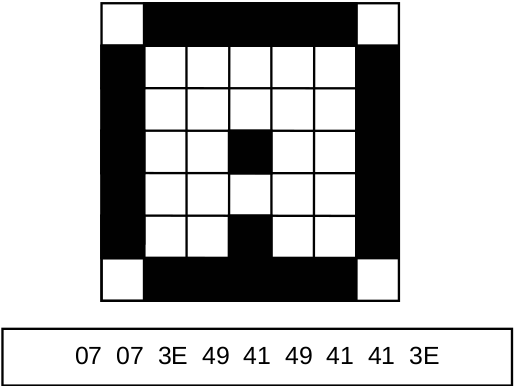
\includegraphics[width=.6\textwidth]{i/b}
	\caption{A pattern and its encoding as an array of bytes (in hex)}
	\label{fig:pattern}
\end{figure}

Some standard patterns are included in module $Display$ and exported as global variables. Among
them are patterns arrow, hook, and star intended to represent the cursor, the caret, and the
marker. A second group of predefined patterns supports drawing graphics.

The parameter $col$ in the pattern-oriented raster operations specifies the pattern's foreground
color. Colors black (background) and white are predefined. Procedure $CopyPattern$ copies the
pattern to location $x$, $y$ in the display area, using the given combination mode. It is probably the
most frequently used operation of all because it is needed to write text. Procedure $ReplPattern$
replicates the given pattern to the given destination block. It starts at bottom left and proceeds
from left to right and from bottom to top. Procedures $Dot$ and $ReplConst$ are special cases of
$CopyPattern$ and $ReplPattern$ respectively, taking a fixed implicit pattern consisting of a single
foreground pixel. $Dot$ is exactly our previously mentioned "set pixel". $ReplConst$ is used to draw
horizontal and vertical lines of various widths.

The raster operations are a prominent example of the use of Oberon's data type $SET$. Formally,
variables are sets of integers between 0 and 31. Here, they are taken as sets of bits numbered
from 0 to 31. We consider the replication of 1's (mode = replace or paint) in the rectangle with
origin $x$, $y$, width $w$, and height $h$. Every line consists of 1024 pixels, or 32 words. al, ar, a0, a1 are addresses.
\begin{verbatim}
  VAR al, ar, a0, a1: INT;
      left, right, pixl, pixr: SET;
  
  al := base + y*128;
  ar := ((x+w-1) DIV 32)*4 + al;
  al := (x DIV 32)*4 + al;
  left  := {(x MOD 32) .. 31};
  right := {0 .. ((x+w-1) MOD 32)};
  FOR a0 := al TO al + (h-1)*128 BY 128 DO
    SYSTEM.GET(a0, pixl);
    SYSTEM.GET(ar, pixr);
    SYSTEM.PUT(a0, pixl + left);
    FOR a1 := a0+4 TO ar-4 BY 4 DO
      SYSTEM.PUT(a1, {0 .. 31});
    END
    SYSTEM.PUT(ar, pixr + right)
  END
\end{verbatim}
The definition (and even more so the implementation) of module $Display$ provides support for a
restricted class of possible hardware configurations only. Any number of display monitors is
theoretically possible. However, they must be mapped to a regular horizontal array of predefined
cells in the display area. Each cell is vertically split into two congruent regions, where the
corresponding monitor is supposed to be able to select and display one of the two regions
alternatively. Finally, it is assumed that all cells hosting black-and-white monitors are allocated to
the left of all cells hosting color monitors. Fig \ref{fig:cell} gives an impression of such a configuration.
\begin{figure}
	\centering
	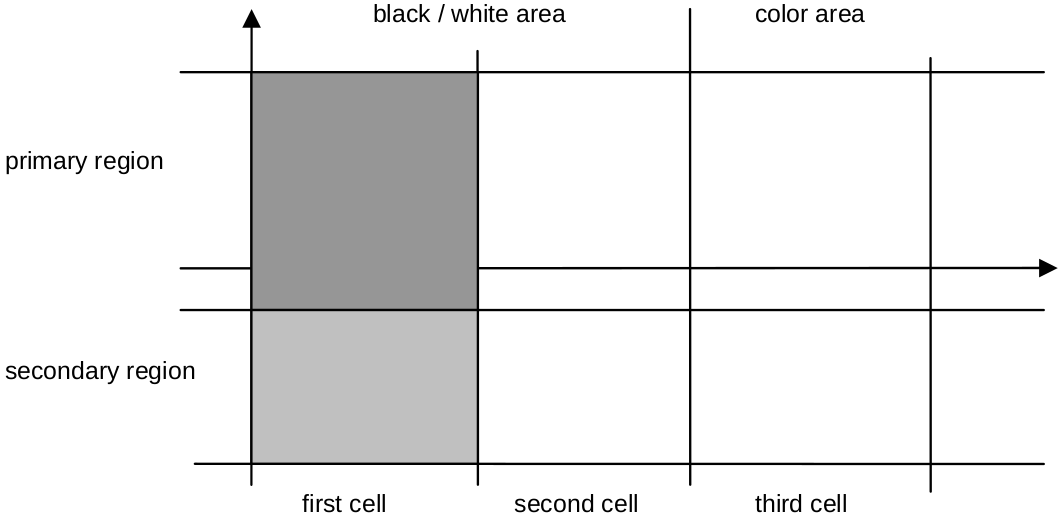
\includegraphics[width=\textwidth]{i/c}
	\caption{General, regular cell structure of display area}
	\label{fig:cell}
\end{figure}

Under these restrictions any concrete configuration can be parameterized by the variables of the
definition above. $Unit$, $Width$, and $Height$ specify the extent of a displayed region, where $Width$ and
$Height$ are width and height in pixel units, and $Unit$ is the size of a pixel in units of 1/36’000 mm.
1/36’000 mm is a common divisor of all of the standard metric units used by the typesetting
community, like mm, inch, Pica point and point size of usual printing devices. $Bottom$ and $UBottom$
specify the bottom y-coordinate of the primary region and the secondary region respectively.
Finally, $Left$ and $ColLeft$ give the left x-coordinate of the area of black-and-white monitors and of
color monitors respectively.

\section{Standard display configs and toolbox}
Let us now take up again our earlier topic of configuring the display area. We have seen that no
specific layout of the display area is distinguished by the general viewer management itself.
However, some support of the familiar standard Oberon display look is provided by module $Oberon$.

In the terminology of this module, a standard configuration consists of one or several horizontally
adjacent displays, where a display is a pair consisting of two tracks of equal height, a user track
on the left and a system track on the right. Note that even though no reference to any physical
monitor is made, a display is typically associated with a monitor in reality.
This is the relevant excerpt of the definition:
\begin{verbatim}
  DEFINITION Oberon;
    PROC OpenDisplay (UW, SW, H: INT);
    PROC OpenTrack (X, W: INT);
    PROC DisplayWidth (X: INT): INT;
    PROC DisplayHeight (X: INT): INT;
    PROC UserTrack (X: INT): INT;
    PROC SystemTrack (X: INT): INT;
    PROC AllocateUserViewer
                 (DX: INT; VAR X, Y: INT);
    PROC AllocateSystemViewer
                 (DX: INT; VAR X, Y: INT);
  END Oberon.
\end{verbatim}
Procedure $OpenDisplay$ initializes and opens a new display of the dimensions $H$ (height), $UW$
(width of user track), and $SW$ (width of system track). Procedure $OpenTrack$ overlays the
sequence of existing tracks spanned by the segment $[X, X + W)$ by a new track. Both procedure
$OpenDisplay$ and $OpenTrack$ take from the client the burden of creating a filler viewer.

The next group of procedures $DisplayWidth$, $DisplayHeight$, $UserTrack$ and $SystemTrack$ return
width or height of the respective structural entity located at position $X$ in the display area.
Procedures $AllocateUserViewer$ and $AllocateSystemViewer$ make proposals for the allocation of a
new viewer in the desired track of the display located at $DX$. In first priority, the location is
determined by the system pointer that can be set manually. If the pointer is not set, a location is
calculated on the basis of some heuristics whose strategies rely on different splitting fractions that
are applied in the user track and in the system track respectively, with the aim of generating
aesthetically satisfactory layouts.

In addition to the programming interface provided by module $Oberon$ for the case of standard
display layouts, the display management section in the $System$ toolbox provides a user interface:
\begin{verbatim}
  DEFINITION System; (*Display management*)
    PROC Open; (*viewer*)
    PROC Close; (*viewer*)
    PROC CloseTrack;
    PROC Recall; (*most recently closed viewer*)
    PROC Copy; (*viewer*)
    PROC Grow; (*viewer*)
    PROC Clear; (*clear system log*)
  END System.
\end{verbatim}
In turn, these commands are called to open a text viewer in the system track, close a viewer,
close a track, recall (and reopen) the most recently closed viewer, copy a viewer, and grow a
viewer. The commands $Close$, $CloseTrack$, $Recall$, $Copy$, and $Grow$ are generic. $Close$, $Copy$, and
$Grow$ are typically included in the title bar of a menu viewer. Their detailed implementations follow subsequently.
